\chapter{Uncertainty and Error Propagation}\label{chap:uncertainty}
Robots are systems that combine sensing, actuation, computation, and communication. Except for computation, all of its sub-systems are subject to a high degree of uncertainty. This can be observed in daily life: phone calls often are of poor quality, making it hard to understand the other party, characters are difficult to read from far away,  the front wheels of your car slip when accelerating on a rainy road from a red light, or your wireless device has a hard time getting a connection. In robotics, measurements taken by on-board sensors are sensitive to changing environmental conditions and subject to electrical and mechanical limitations. Similarly, actuators are not accurate as joints and gears have backlash and wheels do slip. Finally, communication, in particular, wireless either via radio or infrared, is notoriously unreliable.

The goals of this chapter are to understand
\begin{itemize}
\item how to treat uncertainty mathematically using probability theory,
\item how measurements with different uncertainty can be combined,
\item how error propagates when taking multiple measurements in a row.
\end{itemize}

This chapter requires an understanding of random variables, probability density functions, and in particular the Normal distribution. These concepts are explained in a robotic sensing context in Appendix~\ref{sec:pdfs}.

\section{Uncertainty in Robotics as Random Variable}
As quantities such as ``distance to a wall", ``position on the plane'' or ``I can see a blue cross (yes/no)'' are uncertain, we can consider them random variables. A \emph{random variable}\index{Random Variable} can be thought of us the outcome of a ``random'' experiment, such as the face shown when throwing a dice.

Experiments in robotics rarely involve explicit randomness. Instead, sensors are intrinsically noisy due to the physical phenomena associated with them. As sensor readings therefore can be considered random variables, also quantities derived from one or more sensors, such as the examples above, are random variables. This chapter focusses on how to characterize the uncertainty of such aggregated quantities from the uncertainty that characterizes the individual sensors.

\section{Error Propagation}\label{sec:errorprop}
It turns out that the Gaussian Distribution is very appropriate to model prominent random processes in robotics: the robot's position and distance measurements. A differential wheel robot that drives along a straight line, and is subject to slip, will actually increase its uncertainty the farther it drives. Initially at a known location, the expected value (or mean) of its position will be increasingly uncertain, corresponding to an increasing variance. This variance is obviously somehow related to the variance of the underlying mechanism, namely the slipping wheel and (comparably small) encoder noise. Interestingly, we will see its variance grow much faster orthogonal to the robot's direction, as small errors in orientation have a much larger effect than small errors in longitudnal direction. This is illustrated in Figure~\ref{fig:errorprop_odometry}.

\begin{figure}
	\centering
		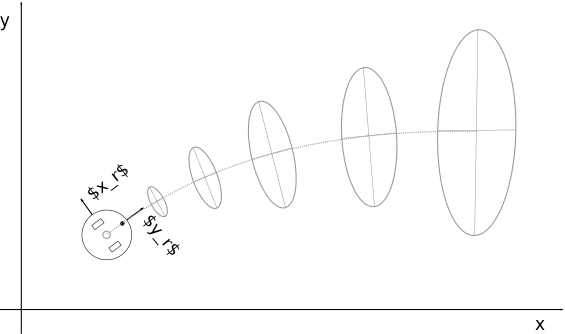
\includegraphics[width=\textwidth]{figs/errorprop_odometry}
	\caption{Two-dimensional Normal distribution depicting growing uncertainty as the robot moves. Albeit starting with equal uncertainty in $x$ and $y$, the large effect of small errors in orientation let the error grow faster in y-direction of the robot.}
	\label{fig:errorprop_odometry}
\end{figure}

Similarly, when estimating distance and angle to a line feature from point cloud data, the uncertainty of the random variables describing distance and angle to the line are somewhat related to the uncertainty of \emph{each} point measured on the line. These relationships are formally captured by the \emph{error propagation law}\index{Error Propagation Law}.

The key intuition behind the error propagation law is that the variance of each component that contributes to a random variable should be weighted as a function of how strongly this component influences this random variable. Measurements that have little effect on the aggregated random variable should also have little effect on its variance and vice versa. ``How strongly'' something affects something else can be expressed by the ratio of how little changes of something relate to little changes in something else. This is nothing else than the partial derivative of something with respect to something else. For example, let $y=f(x)$ be a function that maps a random variable $x$, e.g., a sensor reading, to a random variable $y$, e.g., a feature. Let the standard deviation of $x$ be given by $\sigma_x$. We can then calculate the variance $\sigma_y^2$ by
\begin{equation}
\sigma_y^2=\left(\frac{\partial f}{\partial x}\right)^2 \sigma_x^2
\end{equation}
In case $\mathbf{y}=f(\mathbf{x})$ is a multivariable function that maps $n$ inputs to $m$ outputs, variances become covariance \emph{matrices}. A covariance matrix holds the variance of each variable along its diagonal and is zero otherwise, if the random variables are not correlated. We can then write
\begin{equation}
\Sigma^Y= J \Sigma^X J^T
\end{equation}
where $\Sigma^X$ and $\Sigma^Y$ are the covariance matrices holding the variances of the input and output variables, respectively, and $J$ is a $m$x$n$ \emph{Jacobian} matrix, which holds the partial derivatives $\frac{\partial f_i}{\partial x_j}$. As $J$ has $n$ columns, each row contains partial derivatives with respect to $x_1$ to $x_n$.

\subsection{Example: Line Fitting}\label{sec:linefitting}
Lets consider an example of estimating angle $ \alpha$ and distance $ r$ of a line from a set of points given by $ (\rho_i,\theta_i)$ using Equations~\ref{eq:linealpha}--\ref{eq:liner}. We can now express the relationship of changes of a variable such as $ \rho_i$ to changes in $ \alpha$ by
\begin{equation}
\frac{\partial \alpha}{\partial \rho_i}
\end{equation}
Similarly, we can calculate $ \frac{\partial \alpha}{\partial \theta_i}$, $ \frac{\partial r}{\partial \rho_i}$ and $ \frac{\partial r}{\partial \theta_i}$. We can actually do this, because we have derived analytical expressions for $ \alpha$ and $ r$ as a function of $ \theta_i$ and $ \rho_i$ in Chapter~\ref{chap:feature_extraction}.

We are now interested in deriving equations for calculating the variance of $ \alpha$ and $ r$ as a function of the variances of the distance measurements. Lets assume each distance measurement $ \rho_i$ has variance $ \sigma^2_{\rho_i}$ and each angular measurement $ \theta_i$ has variance $ \sigma^2_{\theta_i}$. We now want to calculate $ \sigma^2_{\alpha}$ as the weighted sum of  $ \sigma^2_{\rho_i}$ and $ \sigma^2_{\theta_i}$, each weighted by its influence on $ \alpha$.
More generally, if we have $ I$ input variables $ X_i$ and $ J$ output variables $Y_j$, the covariance matrix of the output variables $ \sigma_Y$ can be expressed as $\sigma_Y^2=\frac{\partial f}{\partial X}^2 \sigma_X^2$ where $\sigma_X$ is the covariance matrix of input variables and $J$ is a Jacobian matrix of a function $ f$ that calculates $Y$ from $X$ and has the form

\begin{equation}
J=\left[
\begin{array}{ccc}
  \frac{\partial f_1}{\partial X_1} & \ldots & \frac{\partial f_1}{\partial X_I}\\
  \vdots & \ldots & \vdots\\
  \frac{\partial f_J}{\partial X_1} & \ldots & \frac{\partial f_J}{\partial X_I}
 \end{array}
 \right]
\end{equation}

In the line fitting example $ F_X$ would contain the partial derivatives of $ \alpha$ with respect to all $ \rho_i$ (i-entries) followed by the partial derivates of $ \alpha$ with respect to all $ \theta_i$ in the first row. In the second row, $ F_X$ would hold the partial derivates of $ r$ with respect to $ \rho_i$ followed by the partial derivates of $ r$ with respect to $ \theta_i$. As there are two output variables, $ \alpha$ and $ r$, and 2*I input variables (each measurement consists of an angle and distance), $ F_X$ is a 2 x (2I) matrix.

The result is therefore a 2x2 covariance matrix that holds the variances of $ \alpha$ and $ r$ on its diagonal.

\subsection{Example: Odometry}
\screencast{https://www.youtube.com/watch?v=ubg_AAM7Zd8}{errorpropagation}
Whereas the line fitting example demonstrated a many-to-one mapping, odometry requires to calculate the variance that results from multiple sequential measurements.  Error propagation allows us here to not only express the robot's position, but also the variance of this estimate. Our ``laundry list'' for this task looks as follows:
\begin{enumerate}
\item What are the input variables and what are the output variables?
\item What are the functions that calculate output from input?
\item What is the variance of the input variables?
\end{enumerate}

As usual, we describe the robot's position by a tuple $ (x,y,\theta)$. These are the three output variables. We can measure the distance each wheel travels $ \Delta s_r$ and $ \Delta s_l$ based on the encoder ticks and the known wheel radius. These are the two input variables. We can now calculate the change in the robot's position by calculating
\begin{eqnarray}
\Delta x  &=& \Delta s cos(\theta+\Delta \theta /2)\\
\Delta y  &=& \Delta s sin(\theta+\Delta \theta/2)\\
\Delta \theta &=& \frac{\Delta s_r-\Delta s_l}{b}
\end{eqnarray}
with
\begin{equation}
\Delta s=\frac{\Delta s_r + \Delta s_l}{2}
\end{equation}

The new robot's position is then given by
\begin{equation}
f(x,y,\theta,\Delta s_r, \Delta s_l)=[x,y,\theta]^T + [\Delta x \qquad \Delta y \qquad \Delta \theta]^T
\end{equation}
We thus have now a function that relates our measurements to our output variables. What makes things complicated here is that the output variables are a function of their previous values. Therefore, their variance does not only depend on the variance of the input variables, but also on the previous variance of the output variables. We therefore need to write
\begin{equation}\label{eq:errorpropodom}
\Sigma_{p'}=\nabla_p f \Sigma_p \nabla_p f^T + \nabla_{\Delta_{r,l}}f \Sigma_{\Delta}\nabla_{\Delta_{r,l}}f^T
\end{equation}
The first term is the error propagation from a position $ p=[x,y,\theta]$ to a new position $ p'$. For this we need to calculate the partial derivatives of $ f$ with respect to x, y and $ \theta$. This is a 3x3 matrix
\begin{equation}
\nabla_p f=\left[\frac{\partial f}{\partial x} \quad \frac{\partial f}{\partial y} \quad \frac{\partial f}{\partial \theta}\right]=\left[\begin{array}{ccc}1 & 0 & -\Delta s sin(\theta +\Delta \theta /2)\\0 & 1 & \Delta s cos(\theta + \Delta \theta/2)\\0 & 0 &1\end{array}\right]
\end{equation}
The second term is the error propagation of the actual wheel slip. This requires calculating the partial derivatives of $ f$ with respect to $ \Delta s_r$ and $ \Delta s_l$, which is a 3x2 matrix. The first column contains the partial derivatives of $ x,y,\theta$ with respect to $ \Delta s_r$. The second column contains the partial derivatives of $ x,y,\theta$ with respect to $ \Delta s_l$:
\begin{equation}
\nabla_{\Delta_{r,l}} f=\left[
\begin{array}{cc}
\frac{1}{2}\cos(\theta+\Delta \theta/2) & \frac{1}{2}\cos(\theta+\Delta \theta/2)\\
\frac{1}{2}\sin(\theta+\Delta \theta/2) & \frac{1}{2}\cos(\theta+\Delta \theta/2)\\
\frac{1}{2} & -\frac{1}{2}
\end{array}
\right]
\end{equation}

Finally, we need to define the covariance matrix for the measurement noise. As the error is proportional to the distance travelled, we can define $ \Sigma_{\Delta}$ by
\begin{equation}
\Sigma_{\Delta}=\left[\begin{array}{cc}k_r|\Delta s_r| & 0\\0 & k_l|\Delta s_l|\end{array}\right]
\end{equation}
Here $ k_r$ and $ k_l$ are constants that need to be found experimentally and $ |\cdot |$ indicating the absolute value of the distance traveled. We also assume that the error of the two wheels is independent, which is expressed by the zeros in the matrix.

We now have all ingredients for equation~\ref{eq:errorpropodom}, allowing us to calculate the covariance matrix of the robot's pose much like shown in Figure~\ref{fig:errorprop_odometry}.

\section{Take-home lessons}
\begin{itemize}
\item Uncertainty can be expressed by means of a probability density function.
\item More often than not, the Gaussian distribution is chosen as it allows treating error with powerful analytical tools.
\item In order to calculate the uncertainty of a variable that is derived from a series of measurements, we need to calculate a weighted sum in which each measurement's variance is weighted by its impact on the output variable. This impact is expressed by the partial derivative of the function relating input to output.
\end{itemize}

\section*{Exercises}\small
\begin{enumerate}
\item Given two observations $\hat{q}_1$ and $\hat{q}_2$ with variances $\sigma_1$ and $\sigma_2$ of a normal distributed process with actual value $\hat{q}$, an optimal estimate can be calculated by minimizing the expression
\begin{equation}
\nonumber
S=\frac{1}{\sigma_1^2}(\hat{q}-\hat{q}_1)^2+\frac{1}{\sigma_2^2}(\hat{q}-\hat{q}_2)^2
\end{equation}
Calculate $\hat{q}$ so that $S$ is minimized.
\item An ultrasound sensor measures distance $x=c\Delta t/2$. Here, $c$ is the speed of sound and $\Delta t$ is the difference in time between emitting and receiving a signal.
\begin{enumerate}
\item Let the variance of your time measurement $\Delta t$ be $\sigma_t^2$. What can you say about the variance of $x$, when $c$ is assumed to be constant? Hint: how does a change in $\Delta t$ affect $x$?
\item Now assume that also $c$ is changing depending on location, weather, etc.\ and can be estimated with variance $\sigma_c^2$. What is the variance of $x$ now?
\end{enumerate}
\item Consider a unicycle that turns with angular velocity $\dot{\phi}$ and has radius $r$. Its speed is thus a function of $\dot{\phi}$ and $r$ and is given by
\begin{equation}
\nonumber
v=f(\dot{\phi},r)=r\dot{\phi}
\end{equation}
Assume that your measurement of $\dot{\phi}$ is noisy and has a standard deviation $\sigma_{\phi}$.  Use the error propagation law to calculate the resulting variance of your speed estimate $\sigma_v^2$.
\end{enumerate}
\normalsize
